\iffalse
\def\mytitle{PYTHON PROGRAMMING ON MATRICES}
\def\myauthor{K.Pavan Kumar}
\def\contact{r170850@rguktrkv.ac.in}
\def\mymodule{Future Wireless Communication (FWC)}
\documentclass[10pt, a4paper]{article}
\usepackage[a4paper,outer=1.5cm,inner=1.5cm,top=1.75cm,bottom=1.5cm]{geometry}
\twocolumn
\usepackage{graphicx}
\graphicspath{{./images/}}
\usepackage[colorlinks,linkcolor={black},citecolor={blue!80!black},urlcolor={blue!80!black}]{hyperref}
\usepackage[parfill]{parskip}
\usepackage{lmodern}
\usepackage{tikz}
	\usepackage{physics}
\usepackage{tabularx}
\usepackage{enumitem}
\usetikzlibrary{calc}
\usepackage{amsmath}
\usepackage{amssymb}
\renewcommand*\familydefault{\sfdefault}
\usepackage{watermark}
\usepackage{lipsum}
\usepackage{xcolor}
\usepackage{listings}
\usepackage{float}
\usepackage{titlesec}
\providecommand{\mtx}[1]{\mathbf{#1}}
\titlespacing{\subsection}{1pt}{\parskip}{3pt}
\titlespacing{\subsubsection}{0pt}{\parskip}{-\parskip}
\titlespacing{\paragraph}{0pt}{\parskip}{\parskip}


\newcommand{\myvec}[1]{\ensuremath{\begin{pmatrix}#1\end{pmatrix}}}
\let\vec\mathbf
\lstset{
frame=single, 
breaklines=true,
columns=fullflexible
}
\thiswatermark{\centering \put(0,-110.0){
\includegraphics[scale=0.3]{logo.png}} }
\title{\mytitle}
\author{\myauthor\hspace{1em}\\\contact\\FWC22011\hspace{6.5em}IITH\hspace{0.5em}\mymodule\hspace{6em}Matrix:Line}
\date{}
\begin{document}
	\maketitle
	\tableofcontents
	\fi

In parallelogram $ABCD$, two points $\vec{P}$ and $\vec{Q}$ are
taken on diagonal $BD$ such that $DP = BQ$. Show that 
\begin{enumerate}
	\item  $\triangle APD \cong \triangle CQB$         
	\item  $AP = CQ$
	\item $\triangle AQB \cong \triangle CPD$     
	\item  $AQ = CP$   
	\item  $APCQ$ is a parallelogram 
\end{enumerate}
\solution 
See Fig. 
		\ref{fig:9/8/1/9}.
 	\begin{figure}
		\centering
 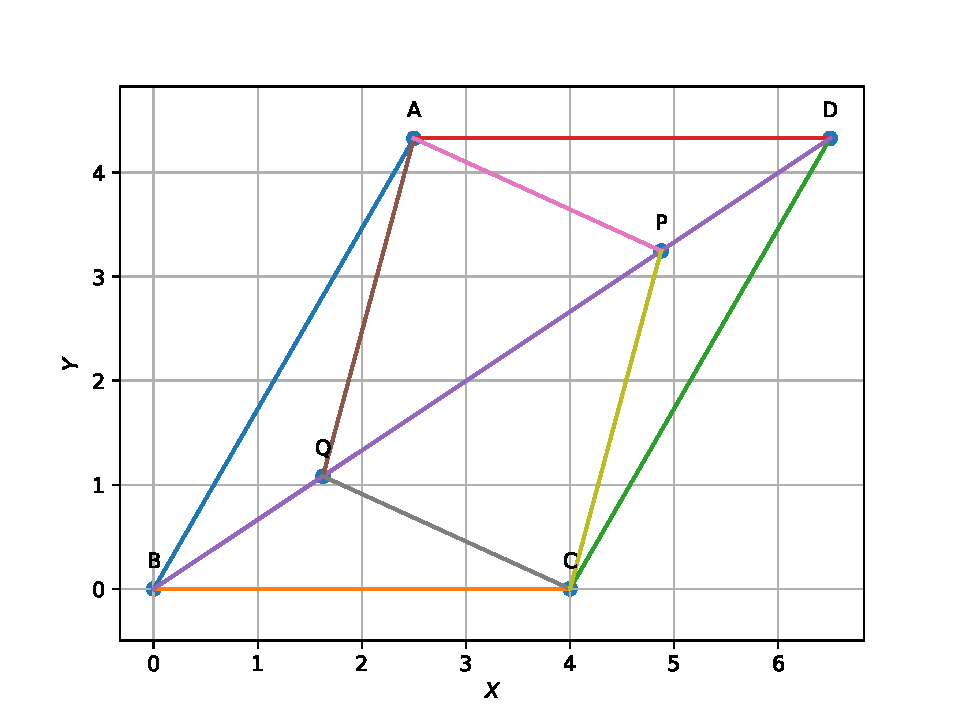
\includegraphics[width=\columnwidth]{chapters/9/8/1/9/figs/output.pdf}
		\caption{}
		\label{fig:9/8/1/9}
  	\end{figure}

\iffalse

\section{Construction}
  	\begin{center}
  Figure of construction
  	\end{center}

   
  \section{Solution}
\begin{center}
The input parameters for this construction are
\begin{tabular}{|c|c|}
	\hline
	\textbf{Symbol}&\textbf{Value}\\
	\hline
	r&5\\
	\hline
	k&3\\
	\hline
    b&4\\
	\hline
	$\theta$&$\frac{pi}{3}$\\
	\hline
\end{tabular}
\end{center}

\begin{align*}
\vec{A}=\begin{pmatrix} r\cos\theta\\ r\sin\theta\ \end{pmatrix} \\
\vec{B}=\begin{pmatrix} 0\\ 0\ \end{pmatrix} \\
\vec{C}=\begin{pmatrix} b\\ 0\ \end{pmatrix} \\
\vec{D}={\vec{A}+\vec{C}-\vec{B}} \\
\vec{P} =  \frac{\vec{B} +K\times \vec{D}}{1+K} \\
\vec{Q} =  \frac{K\times\vec{B} +\vec{D}}{1+K} \\ 
\end{align*}


\textbf{Theorem}\\
A quadrilateral is a parallelogram if a pair of opposite sides
is equal and parallel.

"If two directional vectors are equal,implies their magnitude as well as direction are equal to each other."

Two vectors are parallel if they have the same direction (or) are in exactly opposite directions.

\paragraph{Given} ABCD is a parallelogram.
 ,the two points $\vec{P}$ and $\vec{Q}$ are taken on diagonal BD such that DP = BQ.

\fi
From 
    \eqref{eq:angle2d} and the given information,

\begin{align}
		\label{fig:9/8/1/9/pgm}
	\vec{A}-\vec{B} &=\vec{D}-\vec{C} \\
	\implies    \vec{A}-\vec{D} &=\vec{B}-\vec{C}\\
	\vec{B}-\vec{Q} &=\vec{P}-\vec{D} \quad \text{(given)}
		\label{fig:9/8/1/9/newpgm}
\end{align}

From 
		\eqref{fig:9/8/1/9/pgm}
		and
		\eqref{fig:9/8/1/9/newpgm}
		\iffalse
\begin{align}
\begin{split}
    \vec{A}+\vec{C} =\vec{B}+\vec{D}\\
    \vec{P}+\vec{Q} =\vec{B}+\vec{D}
\end{split}
\end{align}
%From (4)
\begin{align}
    \vec{A}+\vec{C} =\vec{P}+\vec{Q}
\end{align}

From (5)
\fi
\begin{align}
%     \implies  \vec{A}-\vec{Q} =\vec{P}-\vec{C}\\
    \vec{A}-\vec{P} =\vec{Q}-\vec{C}
		\label{fig:9/8/1/9/newpgmsol}
\end{align}


\begin{enumerate}
    \item From 
		\eqref{fig:9/8/1/9/pgm}, 
		\eqref{fig:9/8/1/9/newpgm}
		and 
		\eqref{fig:9/8/1/9/newpgmsol}
		taking the norms of the respective sides, 
    \begin{align}
        \triangle APD \cong \triangle CQB
    \end{align}
    
    \item From 
		\eqref{fig:9/8/1/9/newpgmsol}, taking the norm,
	    \begin{align}
AP=CQ
    \end{align}
    
    \item From 
		\eqref{fig:9/8/1/9/pgm}, 
		\eqref{fig:9/8/1/9/newpgm}
		and 
		\eqref{fig:9/8/1/9/newpgmsol}
		taking the norms of the respective sides, 
    \begin{align}
        \triangle AQB \cong \triangle CPD
    \end{align}

    \item From 
		\eqref{fig:9/8/1/9/newpgmsol}, 
	    \begin{align}
AQ=CP
    \end{align}
\end{enumerate}

\iffalse
     \item Equation (6) and (7) 
      $\implies$  Quadrilateral APCQ is a parallelogram.


\textbf{termux commands :}
\begin{lstlisting}
bash lines.sh............using shell command
\end{lstlisting}
\begin{center}
Below python code realizes the above construction :
\fbox{\parbox{8.5cm}{\url{https://github.com/pavan170850/Fwciith2022/blob/main/matrices/line/code/Line.py}}}
\end{center}
\end{document}
\fi
